% 图 5.6 反铁磁序 = 两套相互贯穿的子晶格之和（5x5 点阵三份，间以 = 与 +）
\documentclass[tikz,border=5pt]{standalone}
\usetikzlibrary{arrows.meta}
\usepackage{amsmath}
\usepackage{bm}
\usepackage{fontspec}
\setmainfont{Times New Roman}
\begin{document}
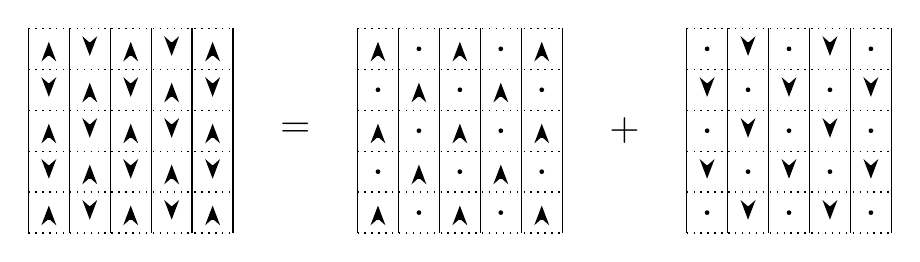
\begin{tikzpicture}[line width=0.8pt,>=Stealth]
\def\s{0.52} % lattice spacing
% ---- macro-like loops via foreach over shifted scopes ----
% panel 1: full checkerboard
\begin{scope}[shift={(0,0)}]
  \foreach \k in {0,...,5}{
    \draw[dotted,line width=0.5] ({-\s/2},{\k*\s-\s/2}) -- ({4*\s+\s/2},{\k*\s-\s/2});
    \draw[line width=0.5] ({\k*\s-\s/2},{-\s/2}) -- ({\k*\s-\s/2},{4*\s+\s/2});}
  \foreach \i in {0,...,4}{\foreach \j in {0,...,4}{
    \pgfmathtruncatemacro{\sg}{mod(\i+\j,2)}
    \ifnum\sg=0
      \draw[->,line width=0.9] ({\i*\s},{\j*\s-0.09}) -- ({\i*\s},{\j*\s+0.09});
    \else
      \draw[->,line width=0.9] ({\i*\s},{\j*\s+0.09}) -- ({\i*\s},{\j*\s-0.09});
    \fi}}
\end{scope}
\node at (4*\s+1.05,4*\s/2) {\Large $=$};
% panel 2: up-sublattice only
\begin{scope}[shift={(4*\s+2.1,0)}]
  \foreach \k in {0,...,5}{
    \draw[dotted,line width=0.5] ({-\s/2},{\k*\s-\s/2}) -- ({4*\s+\s/2},{\k*\s-\s/2});
    \draw[line width=0.5] ({\k*\s-\s/2},{-\s/2}) -- ({\k*\s-\s/2},{4*\s+\s/2});}
  \foreach \i in {0,...,4}{\foreach \j in {0,...,4}{
    \pgfmathtruncatemacro{\sg}{mod(\i+\j,2)}
    \ifnum\sg=0
      \draw[->,line width=0.9] ({\i*\s},{\j*\s-0.09}) -- ({\i*\s},{\j*\s+0.09});
    \else
      \fill ({\i*\s},{\j*\s}) circle (0.030);
    \fi}}
\end{scope}
\node at (4*\s+2.1+4*\s+1.05,4*\s/2) {\Large $+$};
% panel 3: down-sublattice only
\begin{scope}[shift={(8.36,0)}]
  \foreach \k in {0,...,5}{
    \draw[dotted,line width=0.5] ({-\s/2},{\k*\s-\s/2}) -- ({4*\s+\s/2},{\k*\s-\s/2});
    \draw[line width=0.5] ({\k*\s-\s/2},{-\s/2}) -- ({\k*\s-\s/2},{4*\s+\s/2});}
  \foreach \i in {0,...,4}{\foreach \j in {0,...,4}{
    \pgfmathtruncatemacro{\sg}{mod(\i+\j,2)}
    \ifnum\sg=0
      \fill ({\i*\s},{\j*\s}) circle (0.030);
    \else
      \draw[->,line width=0.9] ({\i*\s},{\j*\s+0.09}) -- ({\i*\s},{\j*\s-0.09});
    \fi}}
\end{scope}
\end{tikzpicture}
\end{document}
